%%This is a very basic article template.
%%There is just one section and two subsections.



\documentclass{report}


\usepackage{microtype}
\usepackage[tight,footnotesize]{subfigure}
\usepackage[T1]{fontenc}
\usepackage[latin1]{inputenc} % Input in ISO 8859-1 (Latin1)

\usepackage{ae}               % Almost european, virtual T1-Font
\usepackage[pdftex]{graphicx}
\usepackage{vmargin}          % Adjust margins in a simple way
\usepackage{fancyhdr}         % Define simple headings
\usepackage{subfigure}
\usepackage{url}
\usepackage[absolute,overlay]{textpos}
\usepackage{tikz}
\usepackage[english]{babel}
\usepackage{algorithm}		  % Code-Listings
\usepackage{algorithmic}	  % Code-Listings


\newcommand{\DS}{DynamicSpotter }
\renewcommand*\thesection{\arabic{section}}
\selectlanguage{english}
\begin{document}
\title{\textbf{\DS}\\A Framework for Automatic Diagnosis of Performance Problems\\---\\User
Guide\vspace{100px}}

\author{\textbf{Alexander Wert}\\alexander.wert@kit.edu\\ Am
Fasanengarten 5\\
Software Design and Quality
\\
Karlsruhe Institute of Technology}
\maketitle
\tableofcontents
\newpage


\section{The Approach behind \DS}
\DS is a framework for automatic detection of performance problems in Java-based enterprise software systems. Therefore,
\DS combines the concepts of software performance anti-patterns with systematic experimentation. 

Software performance
anti-patterns (SPAs) \cite{smith2000software,smith2002software,smith2003more,smith2003new} describe common, recurring
design or implementation mistakes leading to impaired software performance. As a big portion of software performance
problems exhibit recurring nature, the concept of SPAs is a means to identify such problems in different
contexts (different target-systems, environments, etc.) by searching for the generic patterns, or characteristics,
different SPAs exhibit. 

If the system under test (SUT) is implemented and can be executed, performance tests allow to
gain insights on its performance behaviour. There are three important things to know about performance tests: 
\begin{enumerate}
  \item Usually, a load driver (such as JMeter\texttrademark \cite{jmeter} or HP LoadRunner \cite{loadrunner}) is used to
generate a set of virtual users processing a script, which describes the work of single users. 
  \item  During
load generation, performance metrics are retrieved from the SUT using instrumentation and monitoring techniques. 
  \item The gathered measurement data is analyzed to provide insights on particular performance engineering tasks.
\end{enumerate}
In our context, the gathered measurement data can be mapped to the
generic characteristics defined by individual SPAs. If measurement data matches certain pattern of an SPA, there is a
high chance that the SUT contains the corresponding anti-pattern. 
However, the following circumstances render the detection of different SPAs with a single performance test impractical.
Different SPAs refer to different parts, performance metrics and granularity levels of the SUT. Thus, in order
to investigate different SPAs in a SUT as part of a single performance test, detailed and excessive instrumentation of
the SUT is required.
However, as each instrumentation instruction comes with a performance overhead, excessive instrumentation yields a
high overhead which distorts measurement data, rendering analysis on this data useless. Hence, an experiment-based
process is needed in which individual SPAs are investigated as part of individual performance tests (in the following
called \emph{experiments}). In this way, during each experiment the SUT is instrumented selectively for the
corresponding SPA, providing detailed measurement data while keeping the performance overhead of the instrumentation
low. 

Though, the experiment-based process significantly mitigates the problem of the performance overhead introduced by the
instrumentation, it increases the manual effort required to configure, execute and analyze each single experiment
referring to an SPA. Moreover, the larger the set of investigated SPAs the more experiments are required, and with that
the time required to execute the experiments grows. However, this problem can be mitigated by using an appropriate
structure of the SPAs. Though there is a large set of different recurring performance problems, many of those problems
share common characteristics and symptoms. Hence, performance problems can be structured in a systematic way, yielding a
hierarchy from high level symptoms to specific root causes of the problems. 
An example of such a hierarchy is depicted in Figure~\ref{fig:hierarchy}.

\emph{Varying Response Times} is a symptom. \emph{The Ramp}~\cite{smith2003new} and \emph{Traffic
Jam}~\cite{smith2002software} are potential causes of \emph{Varying Response
Times}.
\emph{The Ramp} occurs if response times of an application increase during
operation. Such a behaviour can, for example, occur if the
application contains \emph{Dormant References}~\cite{rayside2007object}, i.e.,
the memory consumption of the application is growing over time. The root cause
is \emph{Specific Data Structure}s which are growing during operation or which are not properly
disposed.
The \emph{Traffic Jam} performance antipattern constitutes another cause of \emph{Varying Response Times}. 
A \emph{Traffic Jam} occurs if many concurrent threads or processes are waiting for the same passive resource ((like
semaphores or mutexes)) or active resource (like
CPU or hard disk). In the first case, we have a typical \emph{One Lane Bridge}~\cite{smith2000software}
whose critical resource needs to be identified. We focus on \emph{Synchronization Points}, \emph{Database Locks}, and \emph{Pools} as potential root causes.
In the case of limited physical resources, the root cause can only be a specific \emph{Bottleneck Resource}.
Further examples on a performance problem hierarchy can be found in \cite{wert2013supporting, wert2014automatic,
wert2013performance}. 

A hierarchy as depicted in Figure~\ref{fig:hierarchy} can be utilized as a search
tree, in order to systematically search for performance problems by conducting a depth-first search on the tree. In
particular, a branch or sub-tree of the hierarchy does not need to be investigated if the problem corresponding to the
sub-tree's root node is not present in the SUT. In our example, possible root causes for \emph{The Ramp} do not need to
be investigated if \emph{The Ramp} itself has not been detected in the SUT. In this way, many unnecessary experiments
can be avoided, saving experimentation time and effort. 

\begin{figure}[t]
\subfigure[An exemplary hierarchy of performance problems (from \cite{wert2013supporting}) \label{fig:hierarchy}]{
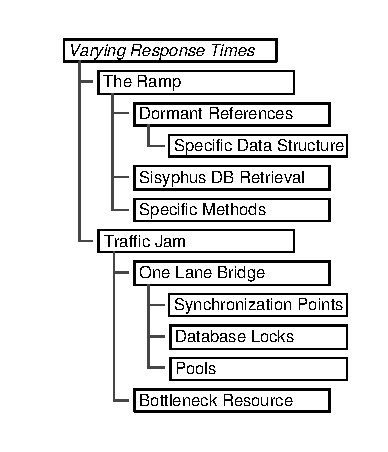
\includegraphics[width=0.3\textwidth]{figures/hierarchy.pdf}
}
\hfill
\subfigure[Overview on the \DS approach (graphic from \cite{wert2014automatic}) \label{fig:spotter}]{
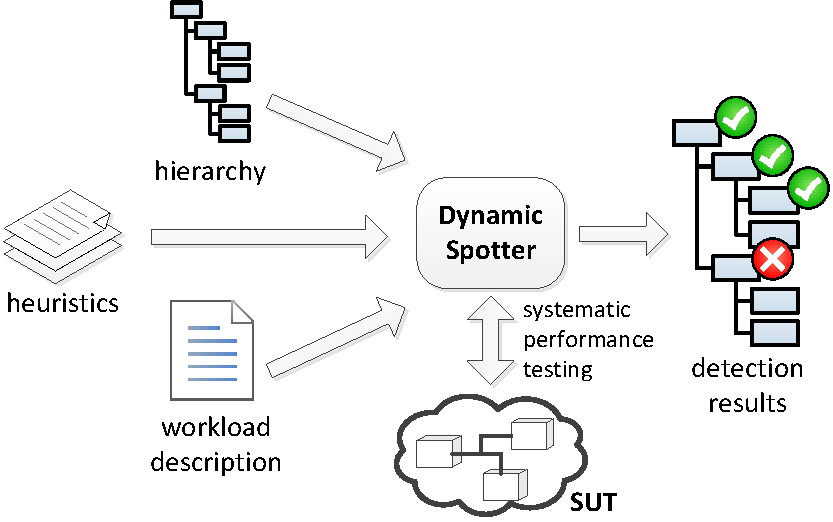
\includegraphics[width=0.6\textwidth]{figures/spotter.pdf}
}
\caption{\DS approach}
\end{figure}

\DS utilizes the concept of hierarchically structuring performance problems (respectively SPAs) in order to automate
the search for recurring performance problems (SPAs) by systematically executing measurement experiments. The high level
approach behind \DS is depicted in Figure~\ref{fig:spotter}. \DS takes a performance problem hierarchy (as described
before) as input. For each node of that hierarchy, performance experts define a heuristic responsible to decide on the
existence of the corresponding problem. To this end, a heuristic executes a series of experiments, observes certain
performance metrics and analyzes them to make a decision. (Note: Both, the hierarchy and the corresponding heuristics
are generic artifacts which do not depend on the SUT under test and, thus, can be reused in other contexts.) For
instance, in order to detect a \emph{One Lane Bridge}, the corresponding heuristic may execute a set of experiments with
different load intensities, while observing end-to-end response times. If response times significantly increase with
the load, while none of the hardware resources is utilized to capacity, the SUT contains an OLB.
For execution of experiments, a load script (\emph{workload description}) specifies the work of single virtual users. 
Traversing the hierarchy and applying corresponding heuristics for each performance problem of the hierarchy, \DS
generates a detection result report. The report states for each node in the hierarchy whether the corresponding
problem exists in the SUT and, where appropriate, points to the root cause and location in the SUT of a detected
problem.



\section{Architecture}
\label{sec:architecture}


\section{DynamicSpotter - Getting Started}
\subsection{Pre-Requisites}
- SUT
- AIM
- resource-sampler
- load-script + load generator

\subsection{Setting up Measurement Environment}
\subsubsection{Starting SUT with an Instrumentation Agent}
\subsubsection{Starting Resource Samplers}
\subsubsection{Setting up a Load Generator Service}


\subsection{Setting up \DS}
\subsubsection{Installation}
\subsubsection{Creating new \DS Project}
\subsubsection{Configuring Spotter}
\subsubsection{Specifying Measurement Environment}
\subsubsection{Specifying Problem Hierarchy}
\subsection{Executing \DS}

\section{Demo Case}

\section{Extending \DS}
\subsection{\DS Extension Mechanism}
\subsection{Detection Controller Extensions}
\subsection{Instrumentation Extensions}
\subsection{Measurement Extensions}
\subsection{Load Generation Adapter Extensions}

\bibliographystyle{IEEEtranSA}
\bibliography{doc}

\end{document}
